\section{Appendix}

% \subsection{Various other scaling plots}
% We next investigate the role various additional hyperparameters play in affecting the performance of each debating strategy.

% \begin{figure}
%   \centering
  
%   % First row: three images side by side
%   \begin{subfigure}[b]{0.3\textwidth}
%     \centering
%     \includegraphics[width=\textwidth]{imgs/ChatEvalDebate_num_rounds.pdf}
%     \caption{ChatEval Rounds}
%   \end{subfigure}
%   \begin{subfigure}[b]{0.3\textwidth}
%     \centering
%     \includegraphics[width=\textwidth]{imgs/EnsembleRefinementDebate_num_reasoning_steps.pdf}
%     \caption{ER Reasoning Steps}
%   \end{subfigure}
%   \begin{subfigure}[b]{0.3\textwidth}
%     \centering
%     \includegraphics[width=\textwidth]{imgs/EnsembleRefinementDebate_num_aggregation_steps.pdf}
%     \caption{ER Aggregation Steps}
%   \end{subfigure}
  
%   % Second row: one image centered
%   \begin{subfigure}[b]{0.3\textwidth}
%     \centering
%     \includegraphics[width=\textwidth]{imgs/MultiAgentDebateTsinghua_max_num_rounds.pdf}
%     \caption{T/S MAD Max Rounds}
%   \end{subfigure}
%   \begin{subfigure}[b]{0.3\textwidth}
%     \centering
%     \includegraphics[width=\textwidth]{imgs/MultiAgentDebateGoogle_num_agents.pdf}
%     \caption{GoogleMAD Agents}
%   \end{subfigure}
%   \begin{subfigure}[b]{0.3\textwidth}
%     \centering
%     \includegraphics[width=\textwidth]{imgs/MultiAgentDebateGoogle_num_rounds.pdf}
%     \caption{GoogleMAD Rounds}
%   \end{subfigure}
  
%   \caption{Metric scaling plots.}
%   \label{fig:metric_correlation}
% \end{figure}

\subsection{Extended results on additional datasets} \label{app:results_overview}
We provide a comprehensive suite of GPT-3 results for each strategy on each dataset: MedQA, PubMedQA, MMLU, CIAR, GPQA, CosmosQA and Chess. 
%, employing various configurations across the three primary datasets: MedQA, PubMedQA, and MMLU. 
For each scenario, we plot accuracy against average time used to answer each question, accuracy relative to average tokens used per question, and accuracy in comparison to the total USD cost. Additionally, a box plot to summarize the performance of each strategy. 
These results can be viewed in Figures \ref{fig:medqa_results}, \ref{fig:pubmedqa_results}, \ref{fig:mmlu_results}, \ref{fig:cosmosqa_results}, \ref{fig:ciar_results}, and \ref{fig:gpqa_results}.

% MedQA
\begin{figure}[h!]
  \centering
  % First row: two images side by side
  \begin{subfigure}[h]{0.49\linewidth}
    \centering
    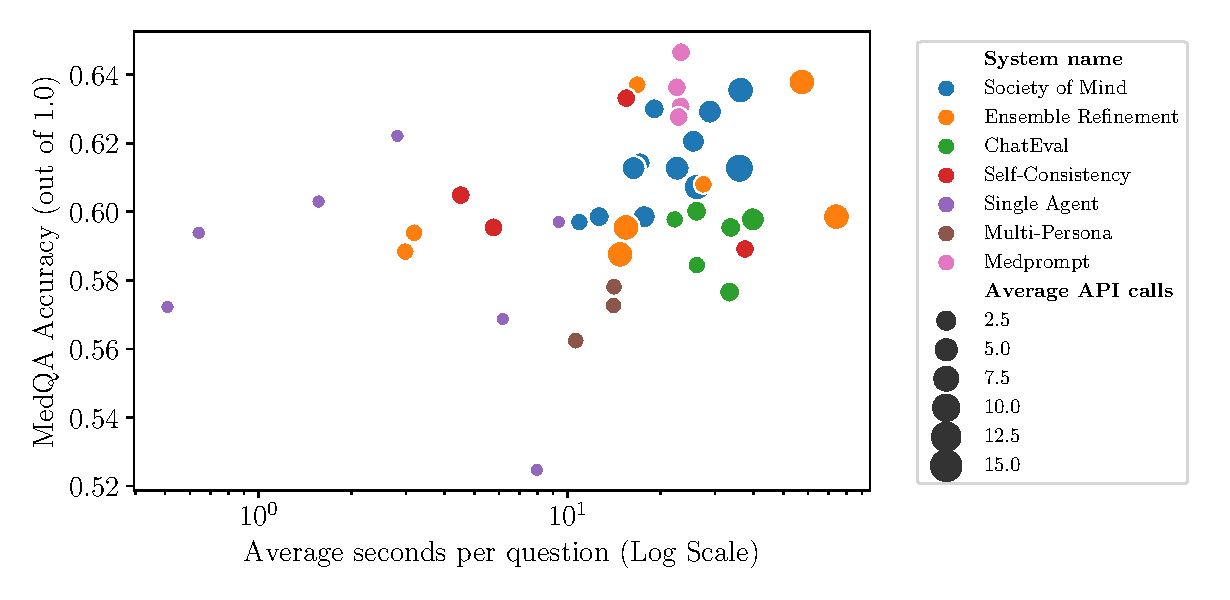
\includegraphics[height=3.9cm, keepaspectratio]{imgs/MedQA_Average_seconds_per_question_scatter_plots.pdf}
    \caption{Accuracy versus the average time per question}
  \end{subfigure}
  \hfill
  \begin{subfigure}[h]{0.49\textwidth}
    \centering
    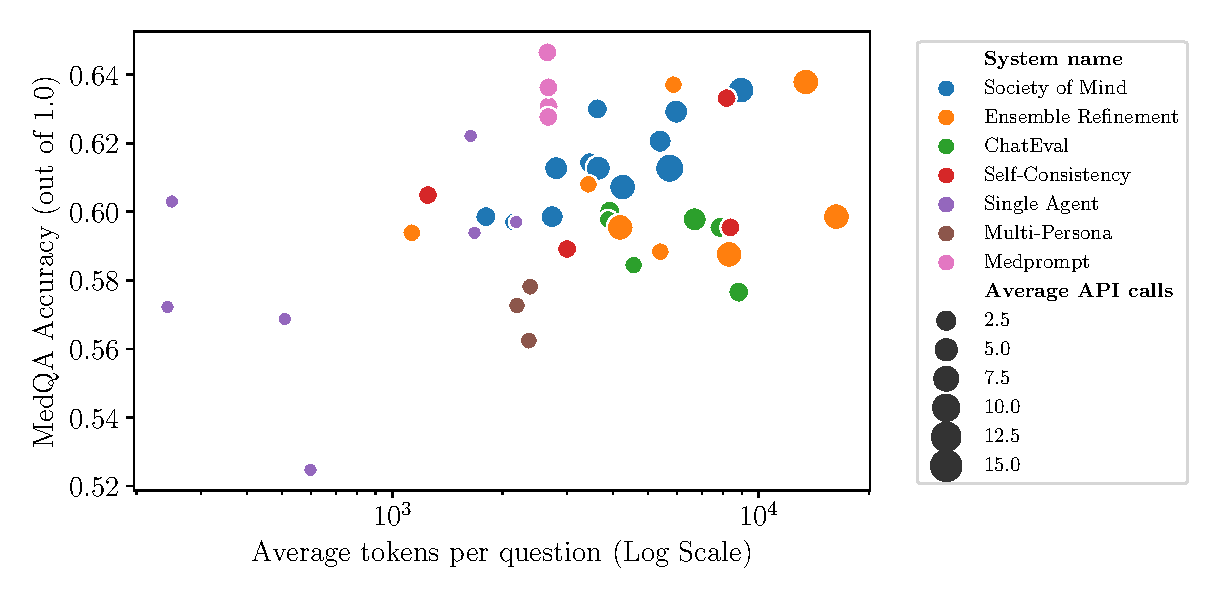
\includegraphics[height=3.9cm, keepaspectratio]{imgs/MedQA_Average_tokens_per_question_scatter_plots.pdf}
    \caption{Accuracy versus Average tokens per question}
  \end{subfigure}
  
  % Second row: two images side by side
  \begin{subfigure}[h]{0.49\textwidth}
    \centering
    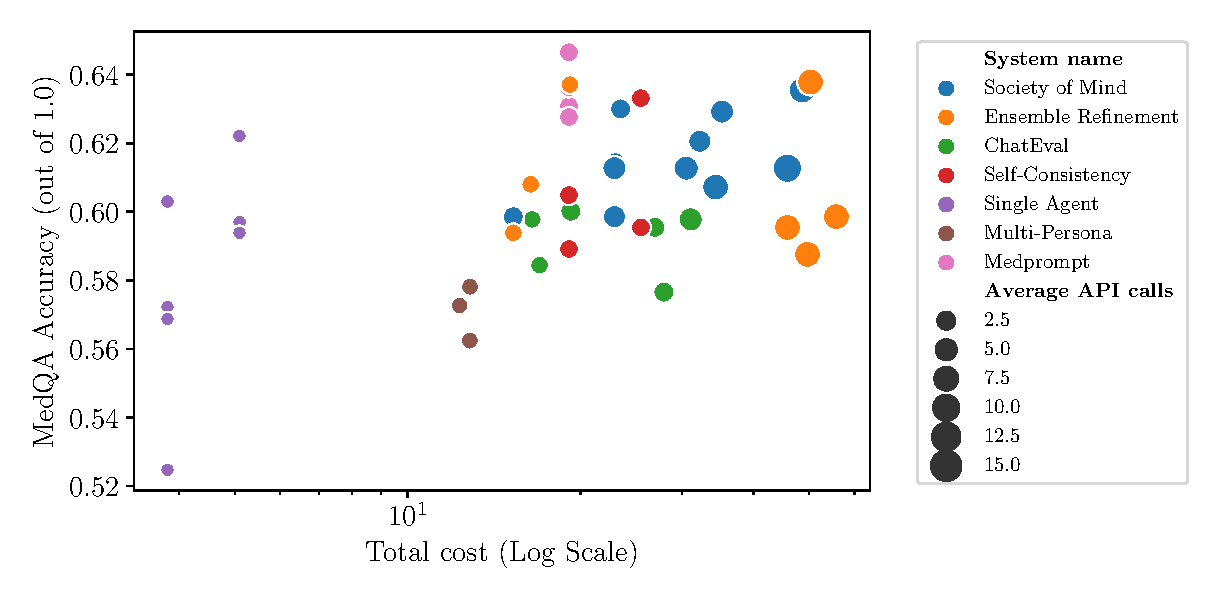
\includegraphics[width=\textwidth]{imgs/MedQA_Total_cost_scatter_plots.pdf}
    \caption{Accuracy versus the total cost}
  \end{subfigure}
  \hfill % Optional, to ensure that there's a little space between the two subfigures
  \begin{subfigure}[h]{0.38\textwidth}
    \centering
    \hspace*{-40mm} % Adjust this value to move the image to the left
    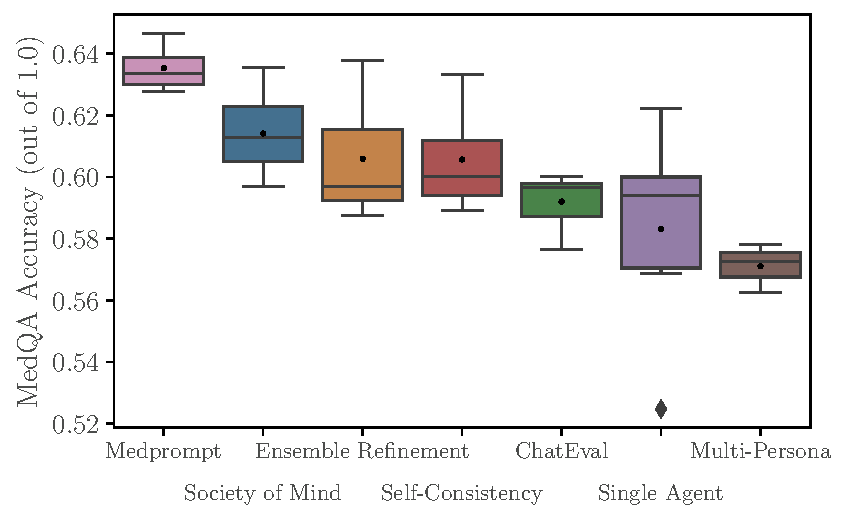
\includegraphics[width=\textwidth]{imgs/medqa_total_acc_box.pdf}
    \caption{Accuracy by strategy}
  \end{subfigure}
\caption{MedQA experimental results.}
\label{fig:medqa_results}
\end{figure}

% PubMedQA
\begin{figure}[H]
  \centering
  % First row: two images side by side
  \begin{subfigure}[h]{0.49\linewidth}
    \centering
    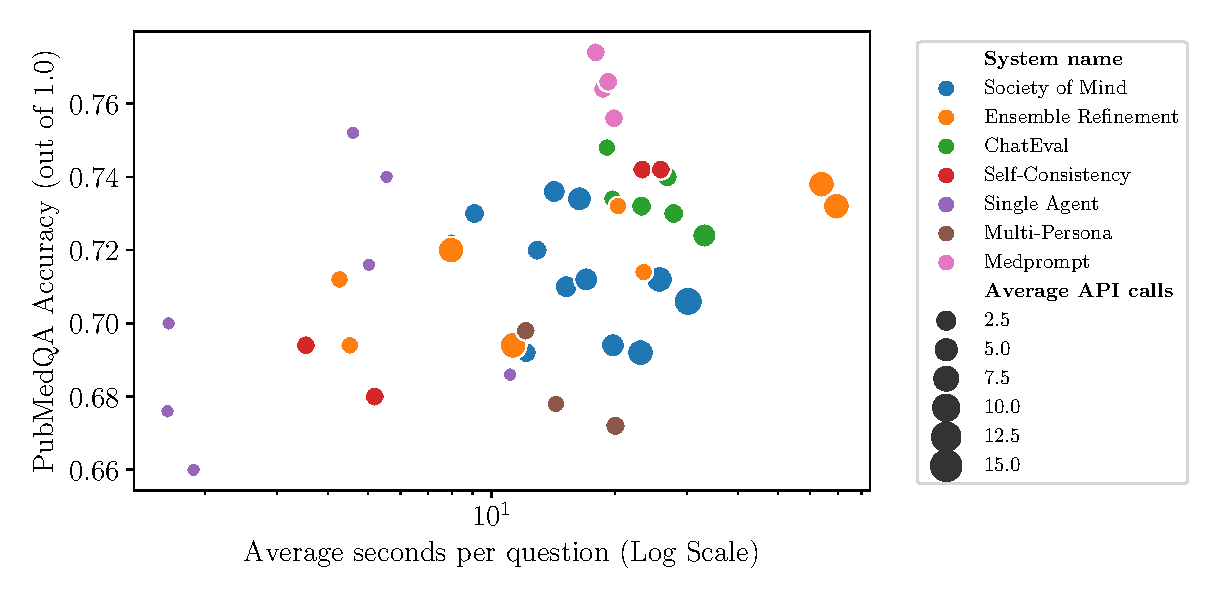
\includegraphics[height=3.9cm, keepaspectratio]{imgs/PubMedQA_Average_seconds_per_question_scatter_plots.pdf}
    \caption{Accuracy versus the average time per question}
  \end{subfigure}
  \hfill
  \begin{subfigure}[h]{0.49\textwidth}
    \centering
    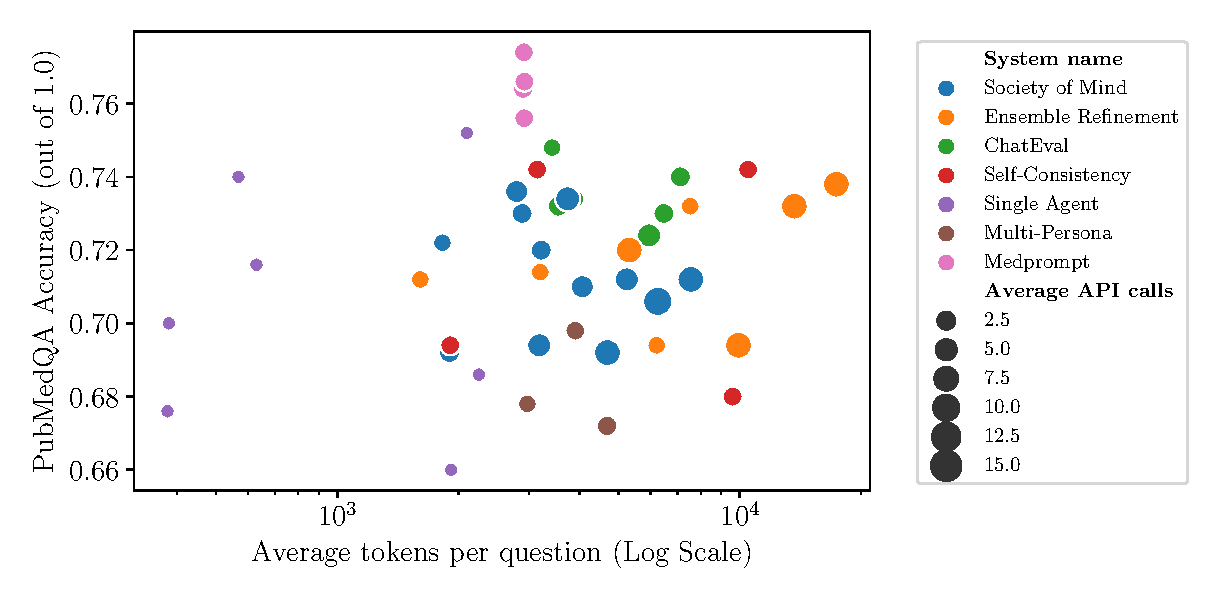
\includegraphics[height=3.9cm, keepaspectratio]{imgs/PubMedQA_Average_tokens_per_question_scatter_plots.pdf}
    \caption{Accuracy versus Average tokens per question}
  \end{subfigure}
  
  % Second row: two images side by side
  \begin{subfigure}[h]{0.49\textwidth}
    \centering
    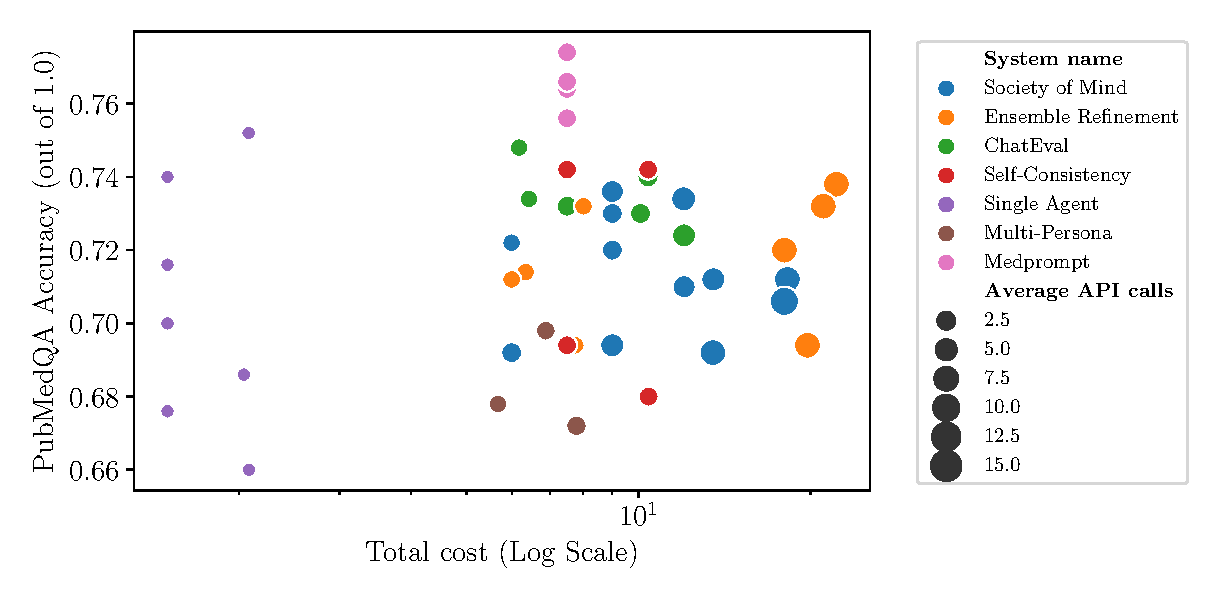
\includegraphics[width=\textwidth]{imgs/PubMedQA_Total_cost_scatter_plots.pdf}
    \caption{Accuracy versus the total cost}
  \end{subfigure}
  \hfill % Optional, to ensure that there's a little space between the two subfigures
  \begin{subfigure}[h]{0.38\textwidth}
    \centering
    \hspace*{-40mm} % Adjust this value to move the image to the left
    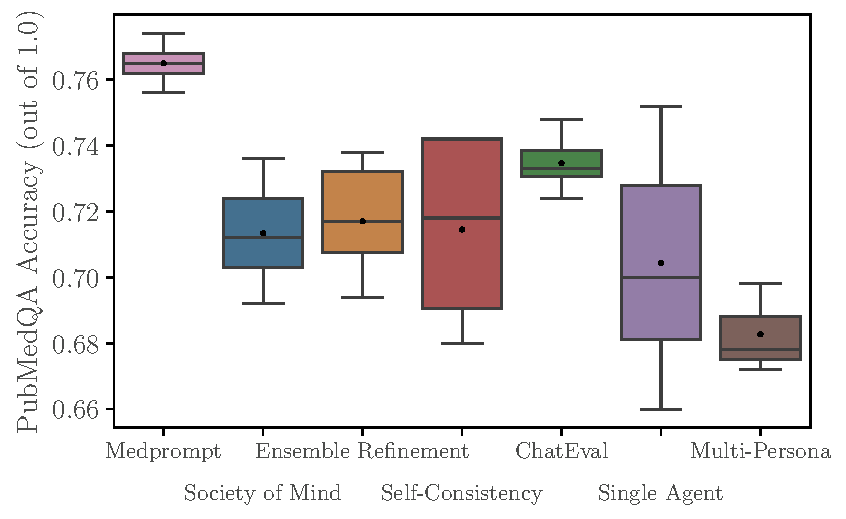
\includegraphics[width=\textwidth]{imgs/pubmedqa_total_acc_box.pdf}
    \caption{Accuracy by strategy}
  \end{subfigure}
\caption{PubMedQA experimental results.}
\label{fig:pubmedqa_results}
\end{figure}

% MMLU
\begin{figure}[H]
  \centering
  % First row: two images side by side
  \begin{subfigure}[h]{0.49\linewidth}
    \centering
    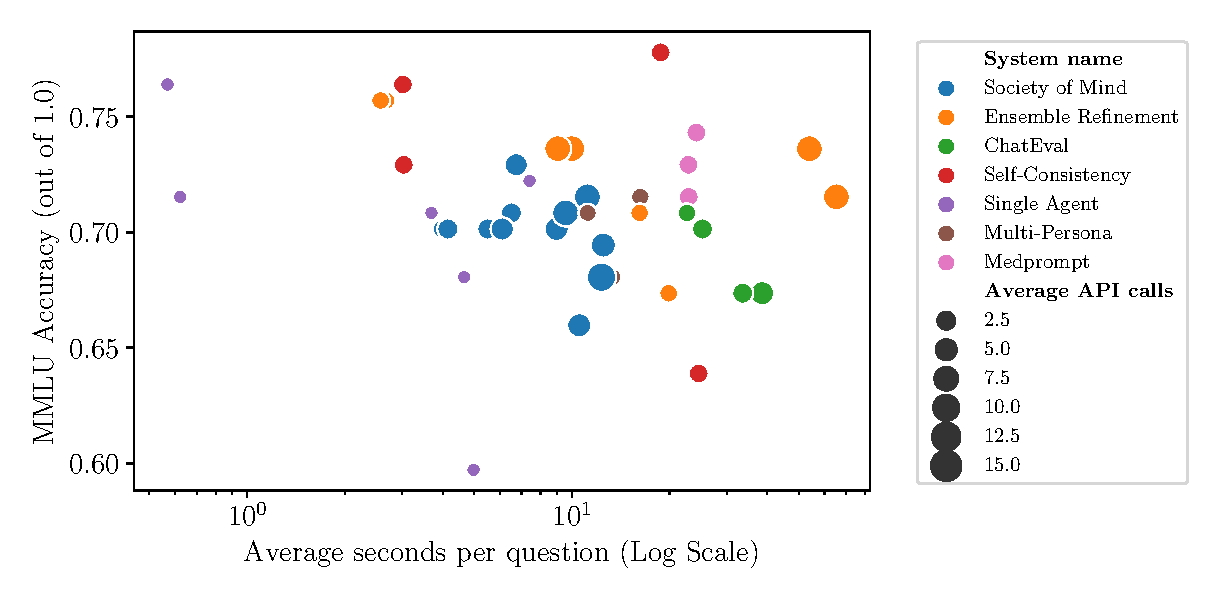
\includegraphics[height=3.9cm, keepaspectratio]{imgs/MMLU_Average_seconds_per_question_scatter_plots.pdf}
    \caption{Accuracy versus the average time per question}
  \end{subfigure}
  \hfill
  \begin{subfigure}[h]{0.49\textwidth}
    \centering
    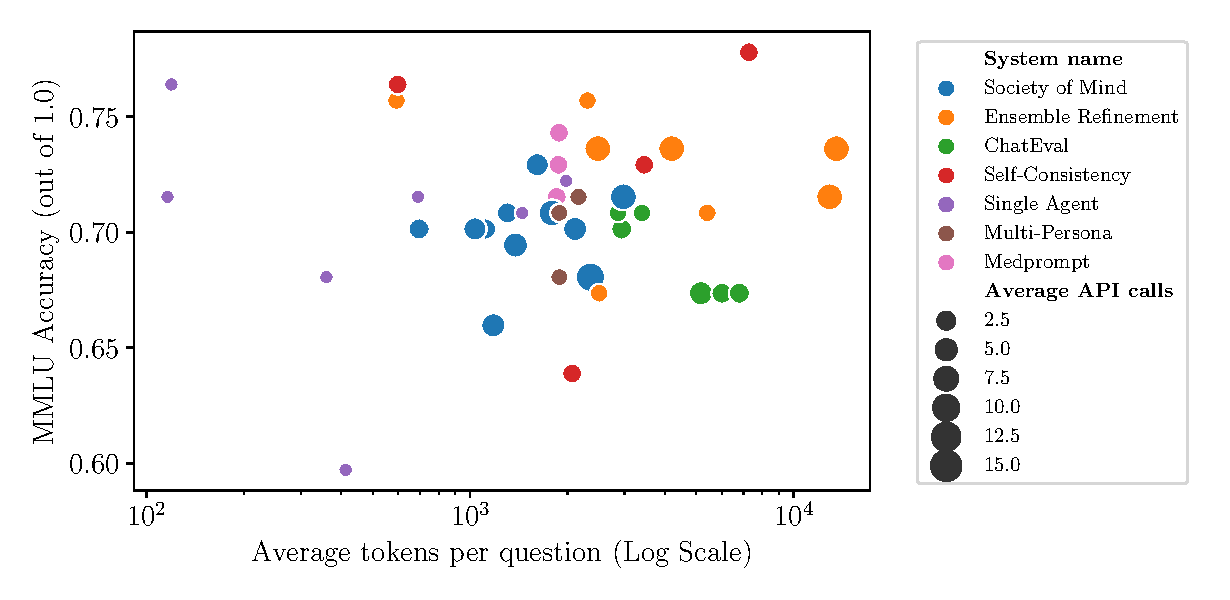
\includegraphics[height=3.9cm, keepaspectratio]{imgs/MMLU_Average_tokens_per_question_scatter_plots.pdf}
    \caption{Accuracy versus Average tokens per question}
  \end{subfigure}
  
  % Second row: two images side by side
  \begin{subfigure}[h]{0.49\textwidth}
    \centering
    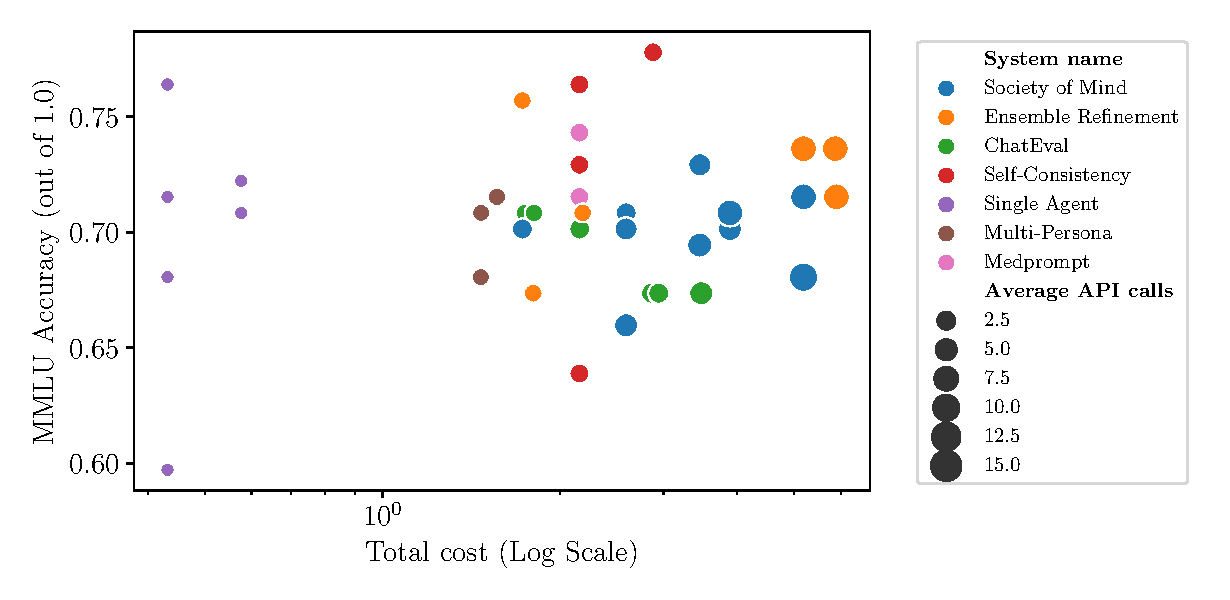
\includegraphics[width=\textwidth]{imgs/MMLU_Total_cost_scatter_plots.pdf}
    \caption{Accuracy versus the total cost}
  \end{subfigure}
  \hfill % Optional, to ensure that there's a little space between the two subfigures
  \begin{subfigure}[h]{0.38\textwidth}
    \centering
    \hspace*{-40mm} % Adjust this value to move the image to the left
    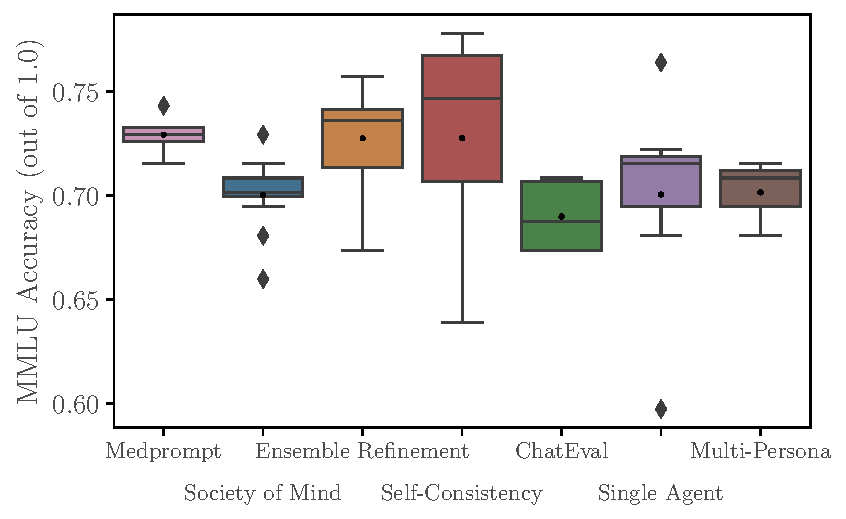
\includegraphics[width=\textwidth]{imgs/mmlu_total_acc_box.pdf}
    \caption{Accuracy by strategy}
  \end{subfigure}
\caption{MMLU experimental results.}
\label{fig:mmlu_results}
\end{figure}

% CosmosQA
\begin{figure}[H]
  \centering
  % First row: two images side by side
  \begin{subfigure}[h]{0.49\linewidth}
    \centering
    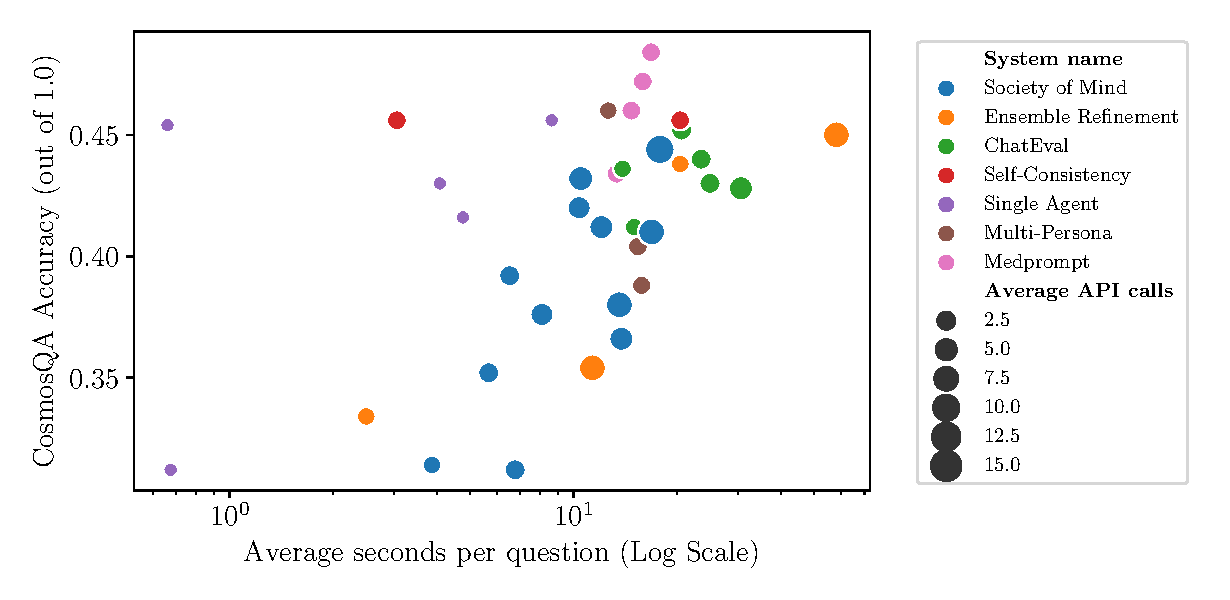
\includegraphics[height=3.9cm, keepaspectratio]{imgs/CosmosQA_Average_seconds_per_question_scatter_plots.pdf}
    \caption{Accuracy versus the average time per question}
  \end{subfigure}
  \hfill
  \begin{subfigure}[h]{0.49\textwidth}
    \centering
    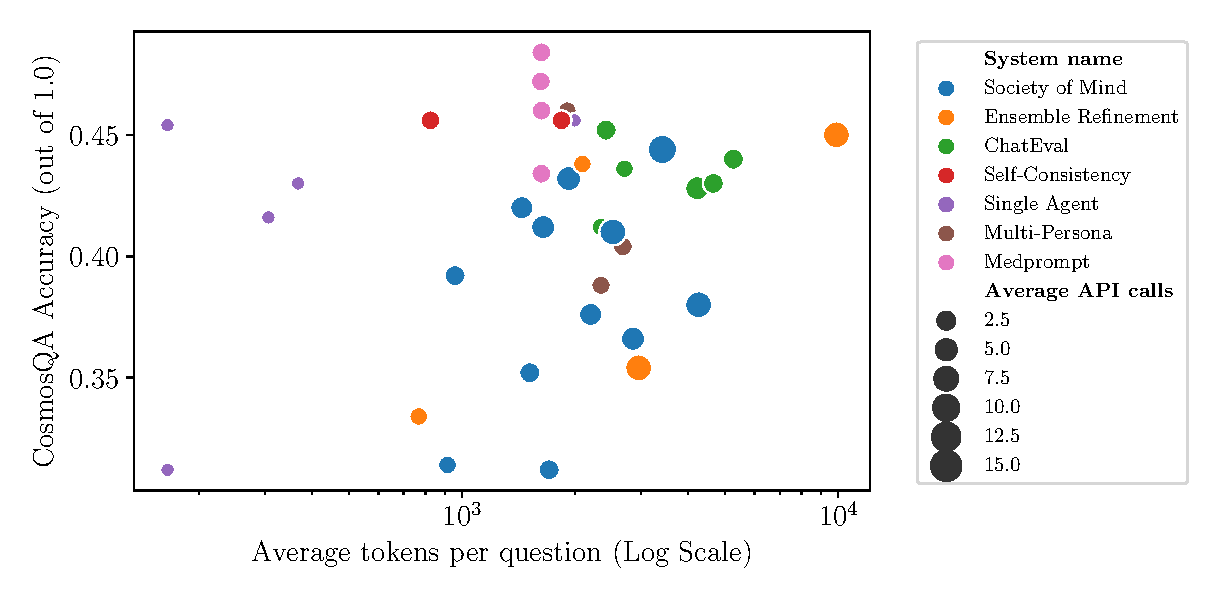
\includegraphics[height=3.9cm, keepaspectratio]{imgs/CosmosQA_Average_tokens_per_question_scatter_plots.pdf}
    \caption{Accuracy versus Average tokens per question}
  \end{subfigure}
  
  % Second row: two images side by side
  \begin{subfigure}[h]{0.49\textwidth}
    \centering
    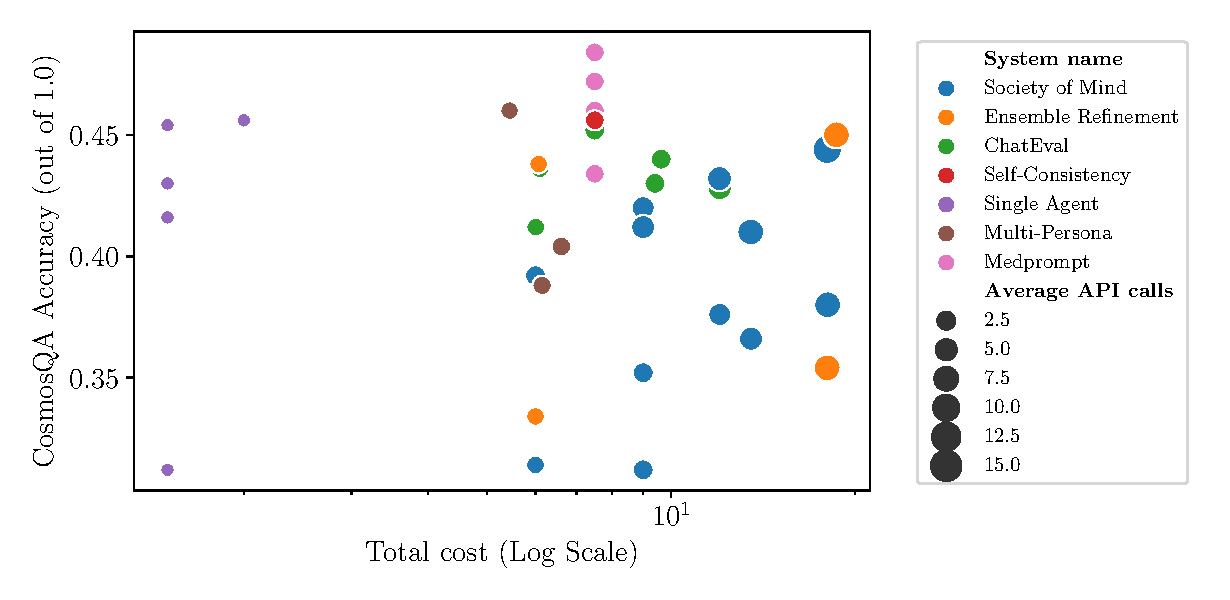
\includegraphics[width=\textwidth]{imgs/CosmosQA_Total_cost_scatter_plots.pdf}
    \caption{Accuracy versus the total cost}
  \end{subfigure}
  \hfill % Optional, to ensure that there's a little space between the two subfigures
  \begin{subfigure}[h]{0.38\textwidth}
    \centering
    \hspace*{-40mm} % Adjust this value to move the image to the left
    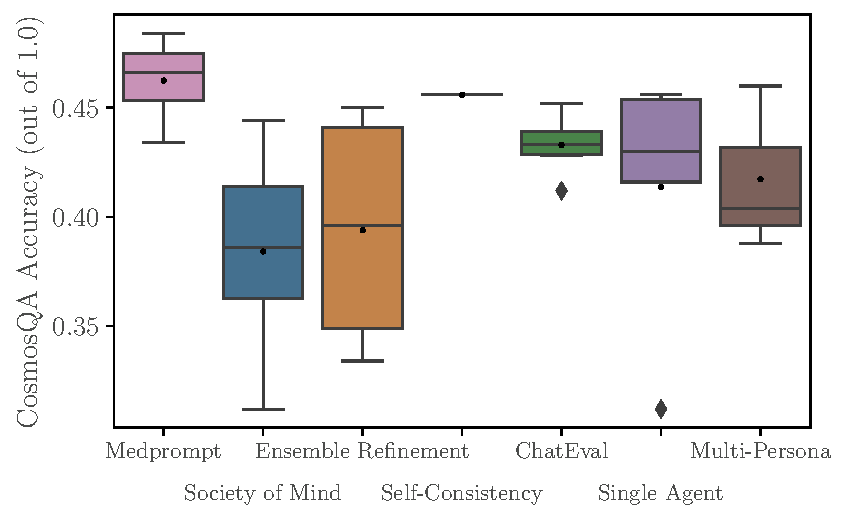
\includegraphics[width=\textwidth]{imgs/cosmosqa_total_acc_box.pdf}
    \caption{Accuracy by strategy}
  \end{subfigure}
\caption{CosmosQA experimental results.}
\label{fig:cosmosqa_results}
\end{figure}

% CIAR
\begin{figure}[H]
  \centering
  % First row: two images side by side
  \begin{subfigure}[h]{0.49\linewidth}
    \centering
    \includegraphics[height=3.9cm, keepaspectratio]{imgs/CIAR_Average_seconds_per_question_scatter_plots.pdf}
    \caption{Accuracy versus the average time per question}
  \end{subfigure}
  \hfill
  \begin{subfigure}[h]{0.49\textwidth}
    \centering
    \includegraphics[height=3.9cm, keepaspectratio]{imgs/CIAR_Average_tokens_per_question_scatter_plots.pdf}
    \caption{Accuracy versus Average tokens per question}
  \end{subfigure}
  
  % Second row: two images side by side
  \begin{subfigure}[h]{0.49\textwidth}
    \centering
    \includegraphics[width=\textwidth]{imgs/CIAR_Total_cost_scatter_plots.pdf}
    \caption{Accuracy versus the total cost}
  \end{subfigure}
  \hfill % Optional, to ensure that there's a little space between the two subfigures
  \begin{subfigure}[h]{0.38\textwidth}
    \centering
    \hspace*{-40mm} % Adjust this value to move the image to the left
    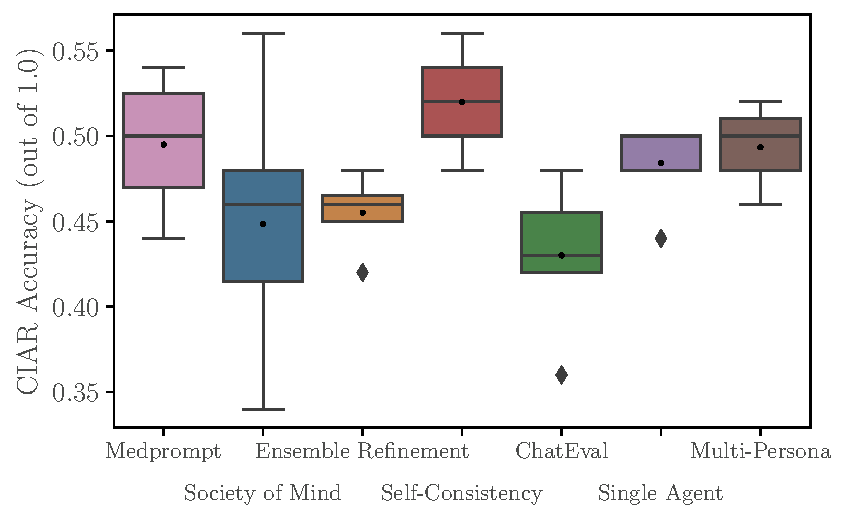
\includegraphics[width=\textwidth]{imgs/ciar_total_acc_box.pdf}
    \caption{Accuracy by strategy}
  \end{subfigure}
\caption{CIAR experimental results.}
\label{fig:ciar_results}
\end{figure}

% GPQA
\begin{figure}[H]
  \centering
  % First row: two images side by side
  \begin{subfigure}[h]{0.49\linewidth}
    \centering
    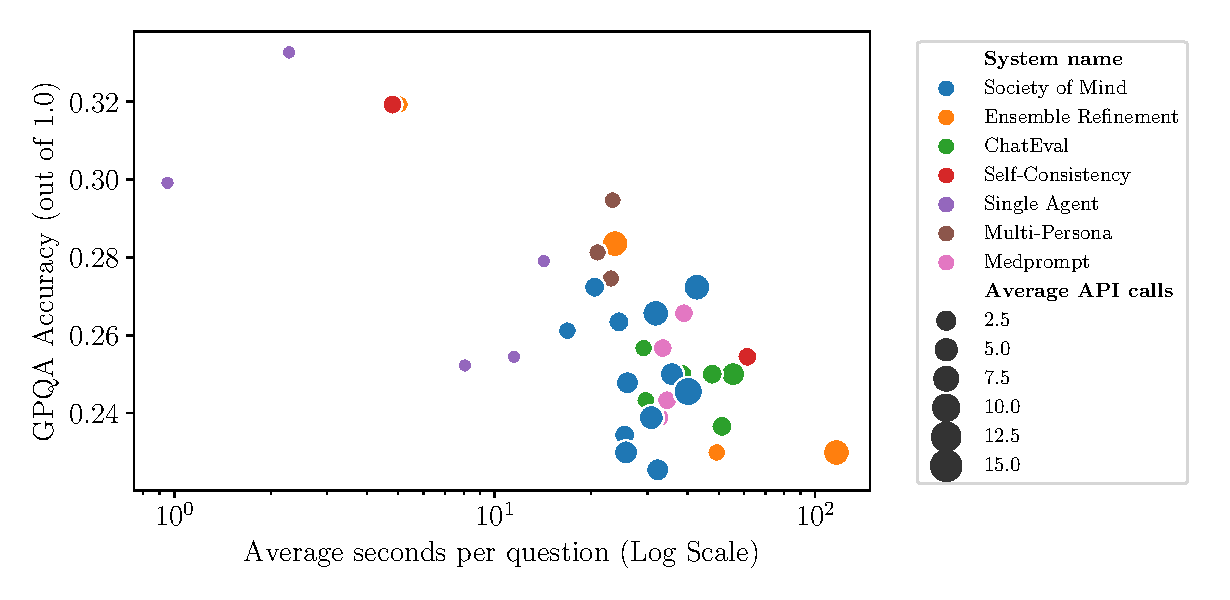
\includegraphics[height=3.9cm, keepaspectratio]{imgs/GPQA_Average_seconds_per_question_scatter_plots.pdf}
    \caption{Accuracy versus the average time per question}
  \end{subfigure}
  \hfill
  \begin{subfigure}[h]{0.49\textwidth}
    \centering
    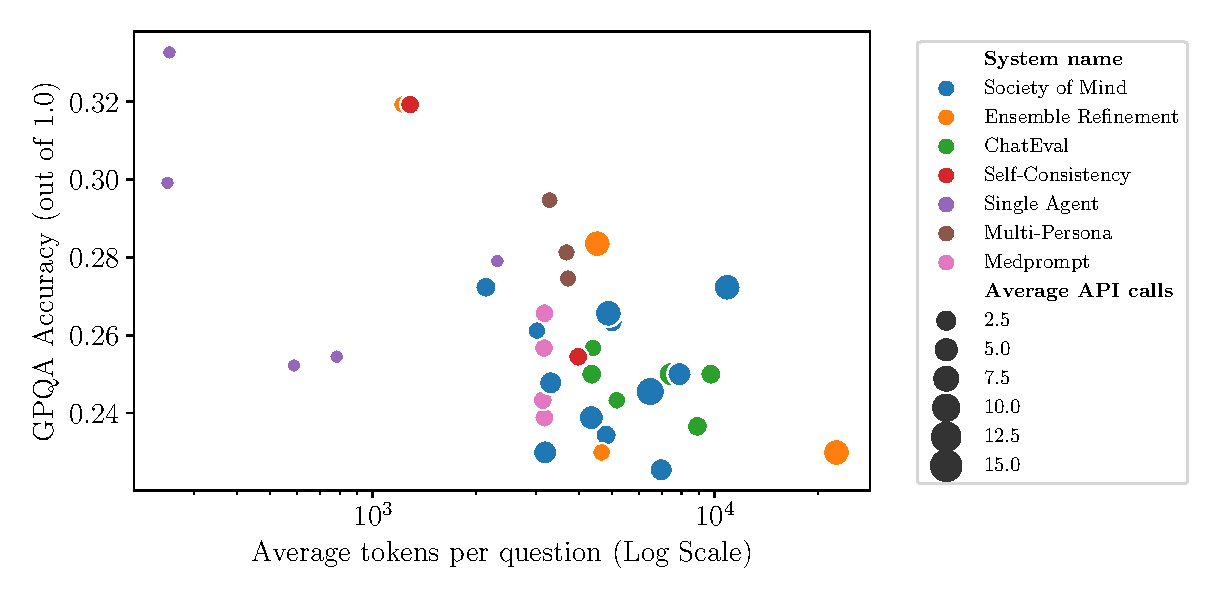
\includegraphics[height=3.9cm, keepaspectratio]{imgs/GPQA_Average_tokens_per_question_scatter_plots.pdf}
    \caption{Accuracy versus Average tokens per question}
  \end{subfigure}
  
  % Second row: two images side by side
  \begin{subfigure}[h]{0.49\textwidth}
    \centering
    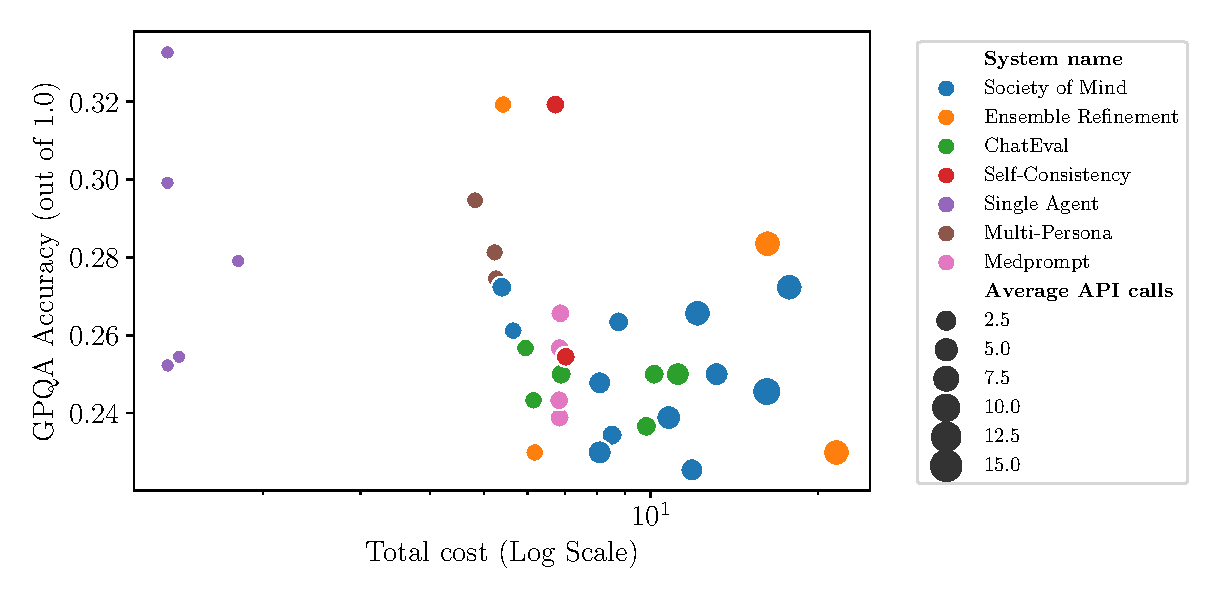
\includegraphics[width=\textwidth]{imgs/GPQA_Total_cost_scatter_plots.pdf}
    \caption{Accuracy versus the total cost}
  \end{subfigure}
  \hfill % Optional, to ensure that there's a little space between the two subfigures
  \begin{subfigure}[h]{0.38\textwidth}
    \centering
    \hspace*{-40mm} % Adjust this value to move the image to the left
    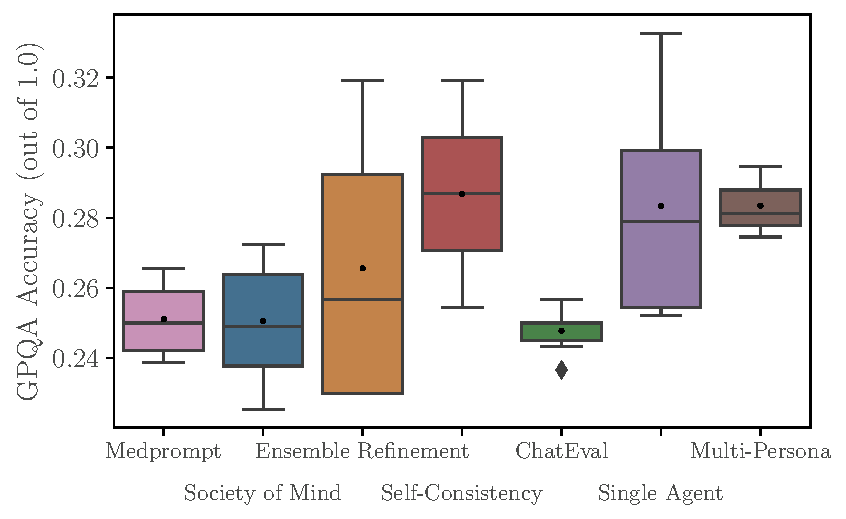
\includegraphics[width=\textwidth]{imgs/gpqa_total_acc_box.pdf}
    \caption{Accuracy by strategy}
  \end{subfigure}
\caption{GPQA experimental results.}
\label{fig:gpqa_results}
\end{figure}

% Chess
\begin{figure}[H]
  \centering
  % First row: two images side by side
  \begin{subfigure}[h]{0.49\linewidth}
    \centering
    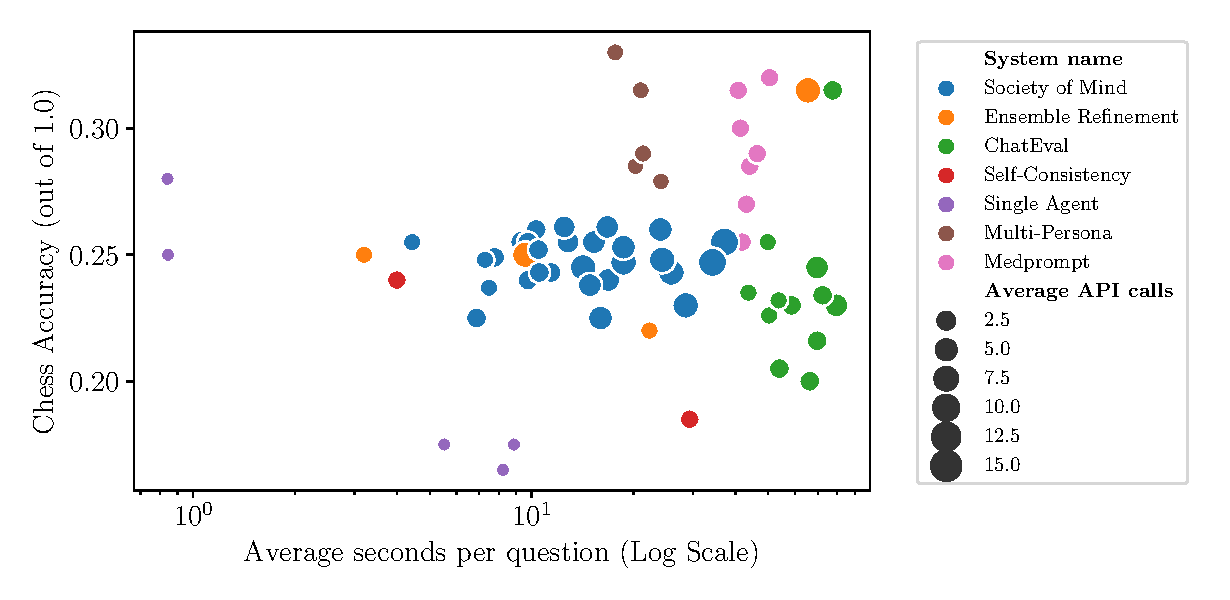
\includegraphics[height=3.9cm, keepaspectratio]{imgs/Chess_Average_seconds_per_question_scatter_plots.pdf}
    \caption{Accuracy versus the average time per question}
  \end{subfigure}
  \hfill
  \begin{subfigure}[h]{0.49\textwidth}
    \centering
    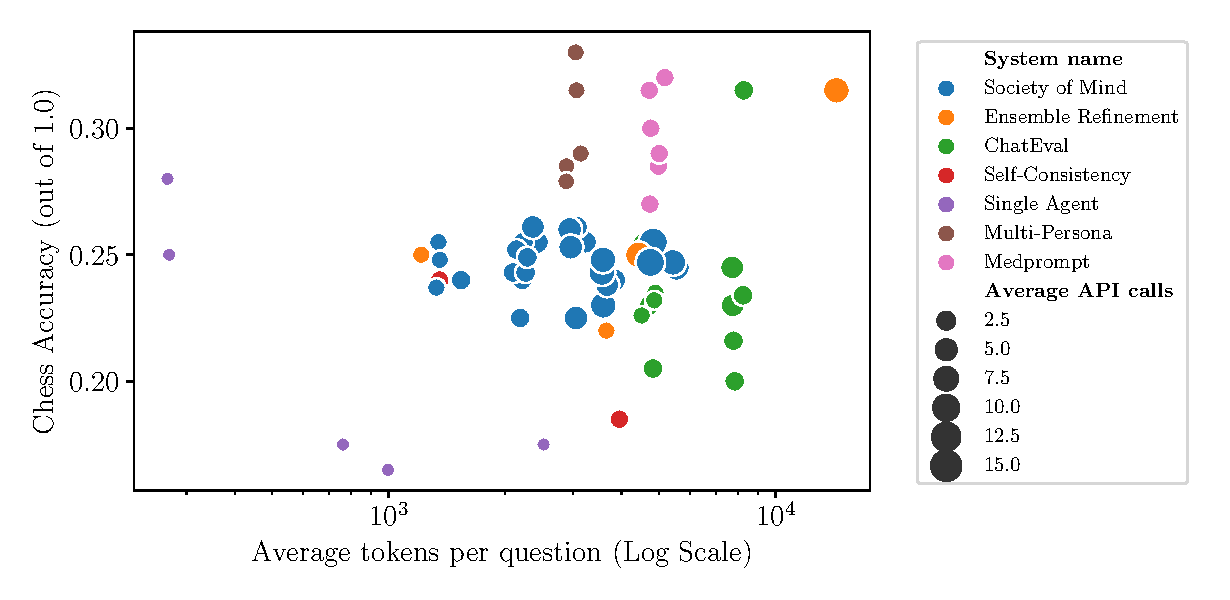
\includegraphics[height=3.9cm, keepaspectratio]{imgs/Chess_Average_tokens_per_question_scatter_plots.pdf}
    \caption{Accuracy versus Average tokens per question}
  \end{subfigure}
  
  % Second row: two images side by side
  \begin{subfigure}[h]{0.49\textwidth}
    \centering
    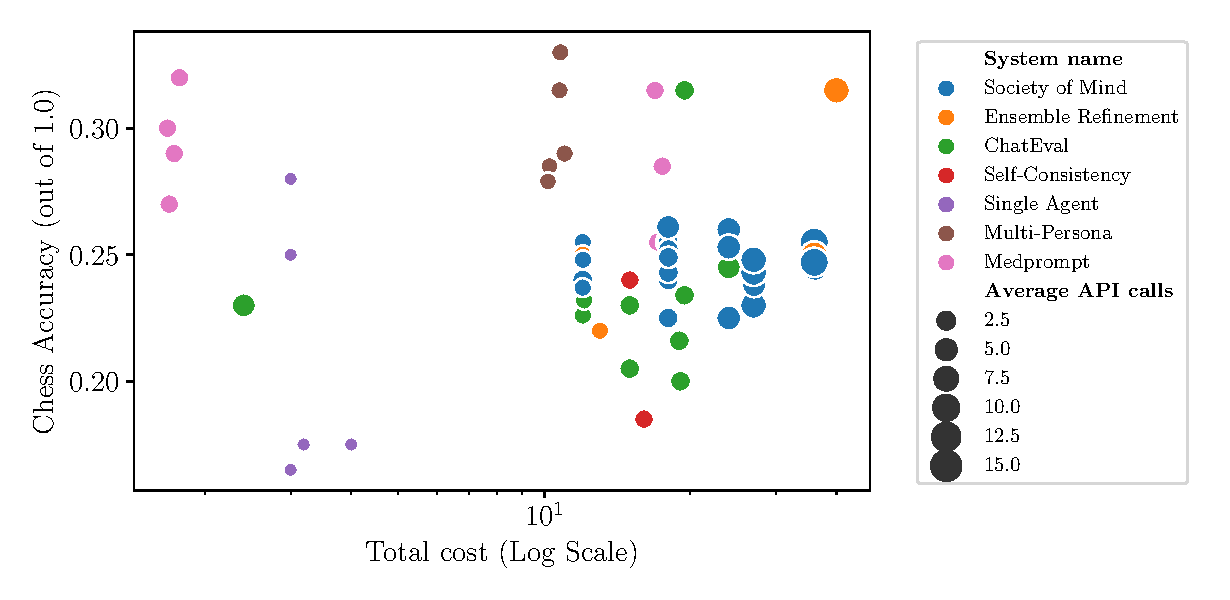
\includegraphics[width=\textwidth]{imgs/Chess_Total_cost_scatter_plots.pdf}
    \caption{Accuracy versus the total cost}
  \end{subfigure}
  \hfill % Optional, to ensure that there's a little space between the two subfigures
  \begin{subfigure}[h]{0.38\textwidth}
    \centering
    \hspace*{-40mm} % Adjust this value to move the image to the left
    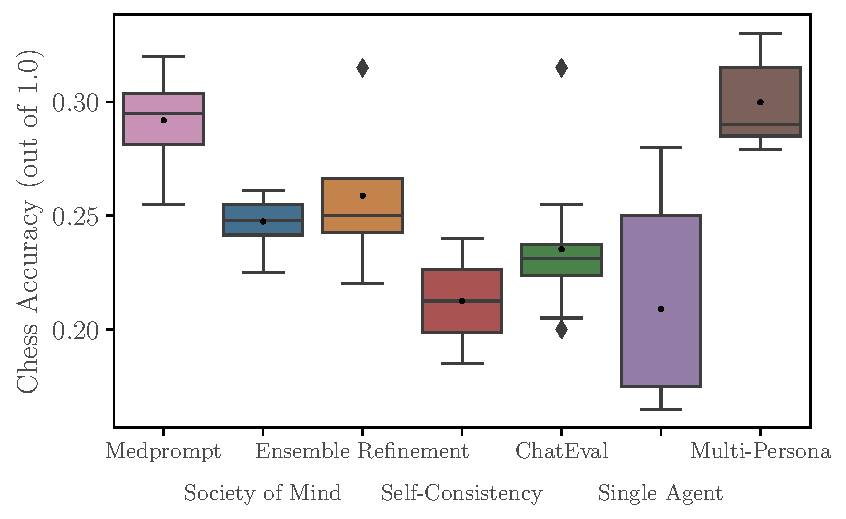
\includegraphics[width=\textwidth]{imgs/chess_total_acc_box.pdf}
    \caption{Accuracy by strategy}
  \end{subfigure}
\caption{Chess experimental results.}
\label{fig:chess_results}
\end{figure}

\newpage\newpage
\subsection{Table of Experiments} \label{app:all_exps}
A complete table of all configurations for each experiment is provided in Table~\ref{app:tab:full-results-table}. This includes the names of the debate and agent prompts used. 
A full description of each of these prompts can be found in Appendix~\ref{app:agent_prompts}.

\small
% \pagenumbering{gobble}
\begin{landscape}

\begin{longtable}{p{2cm}p{1.5cm}p{1cm}p{2.5cm}llllllllllll}
\toprule

System Name & Debate Prompt & Agent prompt & Debate Config &
\multicolumn{2}{c}{MedQA} & \multicolumn{2}{c}{PubMedQA} & \multicolumn{2}{c}{MMLU} & \multicolumn{2}{c}{CosmosQA} & \multicolumn{2}{c}{CIAR} & \multicolumn{2}{c}{GPQA} \\
 &   &    &   & Score & Cost \$ & Score & Cost \$ & Score & Cost \$ & Score & Cost
 \$ & Score & Cost \$ & Score & Cost \$  \\
\midrule
\endhead
\midrule
\multicolumn{10}{r}{Continued on next page} \\
\midrule
\endfoot
\bottomrule
\endlastfoot
Single Agent &   & CoT &  & 0.68 & 0.43 & 0.74 & 1.50 & 0.57 & 3.82 & 0.42 & 1.50 & 0.48 & 0.15 & 0.25 & 1.35 \\
Single Agent &   & CoT &  & 0.60 & 0.43 & 0.72 & 1.50 & 0.52 & 3.82 & 0.43 & 1.50 & 0.44 & 0.15 & 0.25 & 1.41 \\
Single Agent &   & FS + SIMPLE &  & 0.72 & 0.43 & 0.66 & 2.08 & 0.59 & 5.10 &  &  &  &  &  &  \\
Single Agent &   & FS + CoT &  & 0.71 & 0.58 & 0.75 & 2.08 & 0.62 & 5.09 &  &  &  &  &  &  \\
Single Agent &   & SIMPLE &  & 0.76 & 0.43 & 0.70 & 1.50 & 0.60 & 3.82 & 0.45 & 1.50 & 0.50 & 0.15 & 0.33 & 1.35 \\
Single Agent &   & SIMPLE &  & 0.72 & 0.43 & 0.68 & 1.50 & 0.57 & 3.82 & 0.31 & 1.50 & 0.50 & 0.15 & 0.30 & 1.35 \\
ChatEval & CE MAD & CoT & 3 rounds, simultaneous, summarized & 0.67 & 3.48 & 0.72 & 12.02 & 0.60 & 31.10 & 0.43 & 12.01 & 0.42 & 1.21 & 0.25 & 11.19 \\
ChatEval & CE MAD & CoT & 3 rounds, simultaneous talk & 0.67 & 2.86 & 0.73 & 10.08 & 0.60 & 26.95 & 0.43 & 9.41 & 0.46 & 0.97 & 0.24 & 9.82 \\
ChatEval & CE MAD & CoT & 3 rounds, one by one & 0.67 & 2.94 & 0.74 & 10.39 & 0.58 & 27.94 & 0.44 & 9.63 & 0.42 & 1.00 & 0.25 & 10.14 \\
ChatEval & CE MAD & CoT & 2 rounds, simultaneous, summarized & 0.70 & 2.16 & 0.73 & 7.50 & 0.60 & 19.24 & 0.45 & 7.50 & 0.44 & 0.75 & 0.25 & 6.90 \\
ChatEval & CE MAD & CoT & 2 rounds, simultaneous talk & 0.71 & 1.75 & 0.75 & 6.18 & 0.60 & 16.48 & 0.41 & 6.01 & 0.48 & 0.60 & 0.26 & 5.95 \\
ChatEval & CE MAD & CoT & 2 rounds, one by one & 0.71 & 1.81 & 0.73 & 6.43 & 0.58 & 16.97 & 0.44 & 6.10 & 0.36 & 0.62 & 0.24 & 6.15 \\
Ensemble Refinement & ER MAD & FS + SIMPLE & reasoning=3, aggregation=9 & 0.74 & 5.18 & 0.69 & 19.75 & 0.59 & 49.67 &  &  &  &  &  &  \\
Ensemble Refinement & ER MAD & FS + SIMPLE & reasoning=3, aggregation=1 & 0.76 & 1.73 & 0.69 & 7.75 & 0.59 & 19.11 &  &  &  &  &  &  \\
Self-Consistency & ER MAD & FS + SIMPLE &  & 0.73 & 2.16 & 0.68 & 10.42 & 0.60 & 25.48 &  &  &  &  &  &  \\
Ensemble Refinement & ER MAD & SIMPLE & reasoning=3, aggregation=9 & 0.74 & 5.18 & 0.72 & 18.00 & 0.60 & 45.85 & 0.35 & 18.00 & 0.48 & 1.80 & 0.28 & 16.24 \\
Ensemble Refinement & ER MAD & SIMPLE & reasoning=3, aggregation=1 & 0.76 & 1.73 & 0.71 & 6.00 & 0.59 & 15.28 & 0.33 & 6.00 & 0.46 & 0.60 & 0.32 & 5.42 \\
Self-Consistency & ER MAD & SIMPLE &  & 0.76 & 2.16 & 0.69 & 7.50 & 0.60 & 19.10 & 0.46 & 7.50 & 0.56 & 0.75 & 0.32 & 6.73 \\
Ensemble Refinement & ER MAD CoT & CoT & reasoning=3, aggregation=1 & 0.67 & 1.80 & 0.71 & 6.35 & 0.61 & 16.38 & 0.44 & 6.07 & 0.46 & 0.63 & 0.23 & 6.18 \\
Ensemble Refinement & ER MAD CoT & CoT & reasoning=3, aggregation=9 & 0.72 & 5.90 & 0.73 & 21.05 & 0.60 & 55.79 & 0.45 & 18.64 & 0.42 & 2.05 & 0.23 & 21.61 \\
Self-Consistency & ER MAD CoT & CoT &  & 0.64 & 2.16 & 0.74 & 7.50 & 0.59 & 19.10 & 0.46 & 7.50 & 0.48 & 0.75 & 0.25 & 7.03 \\
Ensemble Refinement & ER MAD CoT & FS + CoT & reasoning=3, aggregation=1 & 0.71 & 2.19 & 0.73 & 8.01 & 0.64 & 19.17 &  &  &  &  &  &  \\
Ensemble Refinement & ER MAD CoT & FS + CoT & reasoning=3, aggregation=9 & 0.74 & 5.87 & 0.74 & 22.20 & 0.64 & 50.30 &  &  &  &  &  &  \\
Self-Consistency & ER MAD CoT & FS + CoT &  & 0.78 & 2.88 & 0.74 & 10.40 & 0.63 & 25.47 &  &  &  &  &  &  \\
Multi-Persona & MP MAD & ANGEL + DEVIL & 2 rounds max & 0.68 & 1.47 & 0.68 & 5.68 & 0.57 & 12.32 & 0.46 & 5.44 & 0.50 & 0.48 & 0.29 & 4.83 \\
Multi-Persona & MP MAD & ANGEL + DEVIL & 3 rounds max & 0.71 & 1.47 & 0.70 & 6.88 & 0.56 & 12.83 & 0.39 & 6.15 & 0.46 & 0.47 & 0.28 & 5.23 \\
Multi-Persona & MP MAD & ANGEL + DEVIL & 4 rounds max & 0.72 & 1.57 & 0.67 & 7.79 & 0.58 & 12.84 & 0.40 & 6.61 & 0.52 & 0.50 & 0.27 & 5.26 \\
Medprompt & Medprompt & CoT & temp: 0.5, top p: 0.8 & 0.72 & 2.16 & 0.77 & 7.50 & 0.63 & 19.10 & 0.48 & 7.50 & 0.52 & 0.75 & 0.24 & 6.84 \\
Medprompt & Medprompt & CoT & temp: 0.7, top p: 0.8 & 0.73 & 2.16 & 0.76 & 7.50 & 0.65 & 19.10 & 0.43 & 7.50 & 0.48 & 0.75 & 0.24 & 6.85 \\
Medprompt & Medprompt & CoT & temp: 0.7, top p: 0.5 & 0.73 & 2.16 & 0.76 & 7.50 & 0.63 & 19.10 & 0.46 & 7.50 & 0.54 & 0.76 & 0.26 & 6.85 \\
Medprompt & Medprompt & CoT & temp: 0.5, top p: 0.5 & 0.74 & 2.16 & 0.77 & 7.50 & 0.64 & 19.10 & 0.47 & 7.50 & 0.44 & 0.76 & 0.27 & 6.88 \\
Society of Mind & SoM MAD & CoT & 2 agents, 3 rounds, summarized & 0.66 & 2.59 & 0.69 & 9.00 & 0.61 & 22.92 & 0.41 & 9.00 & 0.48 & 0.90 & 0.23 & 8.09 \\
Society of Mind & SoM MAD & CoT & 4 agents, 3 rounds, summarized & 0.68 & 5.18 & 0.71 & 18.00 & 0.61 & 45.83 & 0.44 & 18.00 & 0.40 & 1.80 & 0.25 & 16.19 \\
Society of Mind & SoM MAD & CoT & 4 agents, 2 rounds, summarized & 0.69 & 3.46 & 0.73 & 12.00 & 0.61 & 30.55 & 0.43 & 12.00 & 0.42 & 1.20 & 0.24 & 10.78 \\
Society of Mind & SoM MAD & CoT & 3 agents, 3 rounds & 0.70 & 3.89 & 0.71 & 13.52 & 0.63 & 35.27 & 0.37 & 13.51 & 0.48 & 1.38 & 0.25 & 13.15 \\
Society of Mind & SoM MAD & CoT & 3 agents, 2 rounds & 0.70 & 2.59 & 0.73 & 9.00 & 0.63 & 23.48 & 0.35 & 9.00 & 0.42 & 0.93 & 0.26 & 8.75 \\
Society of Mind & SoM MAD & CoT & 2 agents, 2 rounds & 0.70 & 1.73 & 0.72 & 6.00 & 0.60 & 15.32 & 0.31 & 6.00 & 0.46 & 0.61 & 0.26 & 5.65 \\
Society of Mind & SoM MAD & CoT & 3 agents, 2 rounds, summarized & 0.70 & 2.59 & 0.74 & 9.00 & 0.60 & 22.91 & 0.42 & 9.00 & 0.52 & 0.90 & 0.25 & 8.09 \\
Society of Mind & SoM MAD & CoT & 2 agents, 2 rounds, summarized & 0.70 & 1.73 & 0.69 & 6.00 & 0.60 & 15.28 & 0.39 & 6.00 & 0.56 & 0.60 & 0.27 & 5.39 \\
Society of Mind & SoM MAD & CoT & 2 agents, 3 rounds & 0.71 & 2.59 & 0.72 & 9.00 & 0.61 & 23.01 & 0.31 & 9.00 & 0.46 & 0.91 & 0.23 & 8.52 \\
Society of Mind & SoM MAD & CoT & 3 agents, 3 rounds, summarized & 0.71 & 3.89 & 0.69 & 13.50 & 0.61 & 34.38 & 0.41 & 13.50 & 0.34 & 1.35 & 0.27 & 12.14 \\
Society of Mind & SoM MAD & CoT & 4 agents, 3 rounds & 0.72 & 5.19 & 0.71 & 18.22 & 0.64 & 48.63 & 0.38 & 18.03 & 0.38 & 1.87 & 0.27 & 17.77 \\
Society of Mind & SoM MAD & CoT & 4 agents, 2 rounds & 0.73 & 3.46 & 0.71 & 12.02 & 0.62 & 32.27 & 0.38 & 12.01 & 0.46 & 1.25 & 0.23 & 11.87 \\

\caption{Complete table of experiment configurations.}\label{app:tab:full-results-table}

\end{longtable}
\end{landscape}




\subsection{Additional Debate Metrics} \label{app:all_debate_metrics}

\begin{tabularx}{\textwidth}{lX} 
    \hline
    \textbf{Metric} & \textbf{Description} \\
    \hline
    Final round consensus & Percentage of agents in agreement with each other at the end of the final round. \\
    % \hline
    Final round correctly parsed consensus & Percentage of agents in agreement with each other at the end of the final round, where we exclude all agents with incorrectly parsed answers. \\
    % \hline
    Any Correct Answer & Percentage of debates where any agent provided the correct answer at least once. \\
    % \hline
    How Many Agents Changed & Number of agents that changed their answer during the debate. \\
    % \hline
    How Many Agents Changed When Correctly Parsed & Number of agents that changed their answer excluding any agents with incorrectly parsed answers. \\
    % \hline
    Number of Rounds & Average number of rounds in the debate. \\
    % \hline
    Unique First Answers & Average number of unique first answers given by the agents. \\
    % \hline
    Unique First Correctly Parsed Answers & Average number of unique first answers excluding incorrectly parsed answers. \\
    \hline
\end{tabularx}

\subsection{Additional Agent Metrics} \label{app:all_agent_metrics}

\begin{tabularx}{\textwidth}{lX}
    \hline
    \textbf{Metric} & \textbf{Description} \\
    \hline
    Agent Engine & The LLM engine used by the agent. \\
    % \hline
    Agent Name & Name of the agent. \\
    % \hline
    Answered Correctly & Percentage of questions answered correctly by the agent. \\
    % \hline
    Any Incorrectly Parsed Answer & Percentage of questions where at least one of the answers were incorrectly parsed. \\
    % \hline
    Avg Messages Removed & Average number of messages removed from the agent's prompt input due to hitting the prompt limit for the LLM model. \\
    % \hline
    Avg Prompt Tokens & Average number of tokens in the prompts given to the agent. \\
    % \hline
    Avg Response Length & Average length of the agent's responses. \\
    % \hline
    Avg Response Tokens & Average number of tokens in the agent's responses. \\
    % \hline
    Avg Round Cost & Average cost for each round of debate for the agent. \\
    % \hline
    Bullied by Other & Percentage of times the agent was bullied by others to change its answer. \\
    % \hline
    Changed Answer & Percentage of times the agent changed its answer througout the debate. \\
    % \hline
    Cost per Question & Average cost incurred by the agent per question. \\
    % \hline
    First Correct Round When Correct & The first round in which the agent gave a correct answer when it was correct. \\
    % \hline
    Incorrectly Parsed Final Answer & Percentage of time when the final answer was parsed incorrectly. \\
    % \hline
    Num of Correct Rounds When Correct & Number of rounds in which the agent was correct when it was correct. \\
    % \hline
    Number of Answers & Average number of unique answers given by the agent throughout a debate. \\
    % \hline
    Percentage of Correct Rounds When Correct & Percentage of rounds in which the agent was correct when it was correct. \\
    % \hline
    Relied on Other & Whether the agent took an answers from another agent in a previous round as its final answer. \\
    % \hline
    Time per Question & Average time taken by the agent per question. \\
    % \hline
    Total Prompt Tokens & Total number of prompt tokens given to the agent. \\
    % \hline
    Total Response Tokens & Total number of tokens in the agent's responses. \\
    % \hline
\end{tabularx}

\newpage
\subsection{Debate Prompts}
\label{app:debate_prompts}
Here we list all the debate-level prompts used in each of the strategies. The prompt names are linked to the entries in the \newline Debate Prompt columns in Table \ref{app:tab:full-results-table}.

% \newgeometry{left=1.5in, right=1.5in}

\tiny
\begin{adjustwidth}{5em}{}
% \fontsize{2}{4}\selectfont
\begin{enumerate}
\item[CE MAD:]

\begin{verbatim}
agent_system_message: You are a debater. Hello and welcome to the medical question answering competition,   
which will be conducted in a debate format. It’s not necessary to fully agree with each other’s perspectives, as our  
objective is to find the correct answer. summarizer_system_message: You are a summarizer. There will be debaters 
involved in a medical question answering debate. Your goal is to summarize the main points in the debate so far,  
which will then be provided to the debaters in the next round.
\end{verbatim}


\item[ER MAD CoT:]
\begin{verbatim}
reasoning_step_message: Instruction: The following are multiple choice questions about medical knowledge. 
Solve them in  a step-by-step fashion, starting by summarizing the available information. Output a single option from  
the four options as the final answer.

aggregation_step_message: The following are multiple choice questions about medical knowledge. Solve them in a 
step-by-step fashion, starting by summarizing the available information. Output a single option from the four options 
as the final answer. We provide several student reasonings for the last question. Some of them may be correct and some 
incorrect. You can use the best correct arguments from these reasonings. Beware of wrong reasoning and do not repeat 
wrong reasoning.
\end{verbatim}

\item[ER MAD:]
\begin{verbatim}
reasoning_step_message: The following are multiple choice questions (with answers) about medical knowledge.

aggregation_step_message: The following are multiple choice questions (with answers) about medical knowledge. We
provide several student reasonings for the last question. Some of them may be correct and some incorrect. You can use 
the best correct arguments from these reasonings. Beware of wrong reasoning and do not repeat wrong reasoning.
\end{verbatim}

\item[SoM MAD:]
\begin{verbatim}
prefix_seperator: \n\n These are the solutions to the problem from other agents: 
summary_prefix_seperator: \n\n These are the main points discussed so far: 

suffix_seperator: \n\n Use these opinions carefully as additional advice, can you provide an updated answer? Make sure 
to state your answer (capital multiple choice letter) at the end of the response.

summary_suffix_seperator: \n\n Use the responses of the experts and carefully provide a summary of the important points 
discussed so far."

agent_response: "\n\n One agent's solution: ```{}```
\end{verbatim}

% \item[SIMPLE:]
% \begin{verbatim}
% You are a helpful medical expert tasked with answering a multiple-choice medical question. You will be conversing with other
% medical experts with the goal of finding the correct answer together. If you find that your previous suggested answer was wrong, you will 
% happily
% update your answer. But you will also point out errors in others’ reasoning.
% \end{verbatim}

\item[MP MAD:]
\begin{verbatim}
agent_system_message: You are a debater. Hello and welcome to the medical question answering competition, which will be 
conducted in a debate format. It’s not necessary to fully agree with each other’s perspectives, as our objective is to 
find the correct answer. The debate topic is to give the correct answer to the following question: \n\n{question}.

judge_system_message: You are a moderator. There will be two debaters involved in a debate. They will present their 
answers and discuss their perspectives on the following question: \n{question}.
\n\nAt the end of each round, you will evaluate answers and decide which is correct.

suffix_seperator: \n\n Use these opinions carefully as additional advice, can you provide an updated answer? Make 
sure to state your answer (capital multiple choice letter) at the end of the response.
\end{verbatim}
\item[Medprompt:]
\begin{verbatim}
system: You are a helpful assistant that answers multiple choice questions about medical knowledge.
\end{verbatim}
\end{enumerate}
\end{adjustwidth}

\newpage
\subsection{Agent Prompts}
\label{app:agent_prompts}
\input{prompts/agent}

